\chapter*{Introduction}

The world of High Performance Computing (HPC) will reach another milestone in the power of machine with Exascale. 
The United States of America and Europe will reach Exascale capability by 2020 or 2021, but China may have the power by 2019. 

%In the aurora 2020-2021 for United States of America and Europe and maybe before, like 2019, for China, the world of High Performance Computing (HPC) will reach another milestone in the power of machines: the Exascale. 
These supercomputers will be $100$ times faster than the estimated overall operations performed by the human brain and its $10^{16}$ \textbf{FL}oating point \textbf{O}perations \textbf{P}er \textbf{S}econd (FLOPS) \cite{kurzweil2010singularity} and achieve a computational power of a quintillion of ($10^{18}$) FLOPS.
This odyssey began with the first vacuum tubes computers and the need of ballistic computation for war. 
Nowadays, supercomputers extended their fields of application and the power of a nation is represented not only by its army and money, but also by the computational power of its supercomputers.
HPC's applications has now spread into all the area of science and technology.\\

Since 1962, considering the Cray CDC 6600 as the first supercomputer, the power of these machines has increased following an observation of the co-founder of the Intel company, Gordon Moore. 
Better known under the name of "Moore's Law", it speculates in 1965 that, considering the constant evolution of technology, the number of transistors on a dense integrated circuit will double approximately every two years. 
Thus, the computational power, that intrinsically depends on the number of transistors on the chip, will increase.
More importantly, as "\textit{money is the sinews of war}", the cost of the die for the same performances will decrease.  
This observation can be compared to the supercomputers results throughout the years in the TOP500 list. 
As presented on figure~\ref{fig:intro_top500} the Moore's law appears to be accurate and sustainable even though it was estimated in early 1965. 

\begin{figure}
\centering
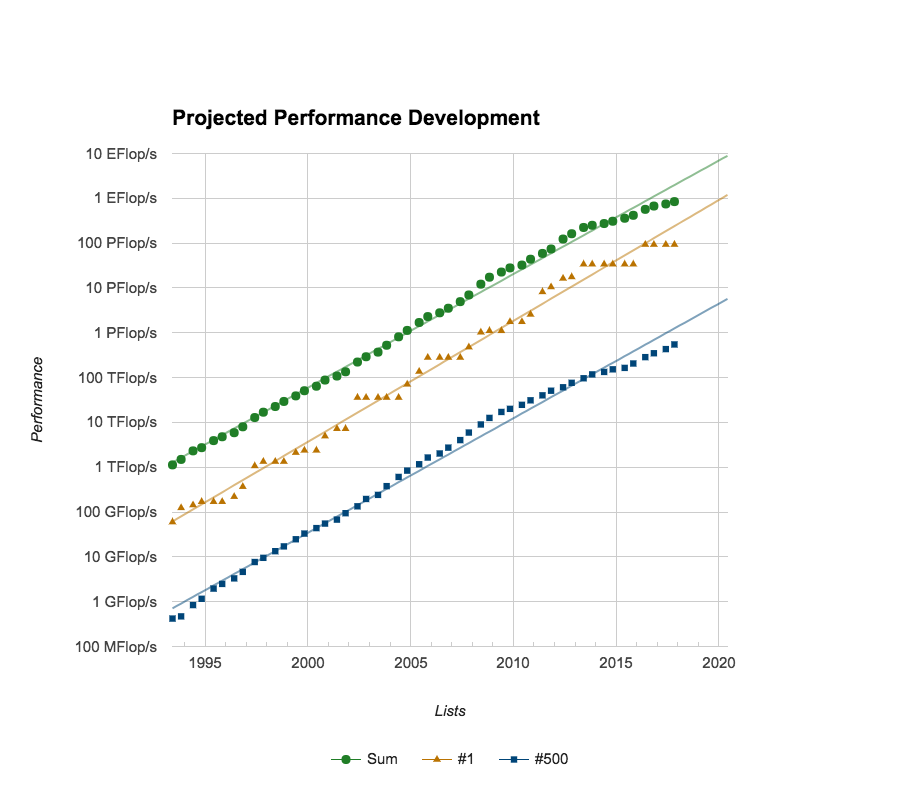
\includegraphics[width=.85\linewidth]{figures/introduction/top500_list_approximation.png}
\caption{Computational power evolution in the TOP500 list}
\label{fig:intro_top500}
\end{figure}

The shrink in the semiconductor with smaller transistors was not the only driver of the linear evolution.
The first one-core Central Processing Units (CPUs) were made using more transistors and had a faster frequency.
They later faced limitations to reach high frequencies because of the power consumption and the inherent cooling of the heat generated by the chip.
This is why IBM proposed the first multi-core processor on the same die, the Power4, in early twentieth century.
The constructors started to create chips with more than one core to increase the computational power in conjunction with the shrink of semiconductors, answering the constant demand of more powerful devices and allowing the Moore's law to thrive. 
This increase of the overall power of the chip comes with some downside, such as costs in synchronizations steps between the cores for memory access, work sharing and complexity.
Currently, the general-purpose CPU features from two to less than a hundred of cores on a single chip.\\

In order to reach even more computational power some researchers started to use many-core approaches. 
By using hundreds of cores, these devices take advantage of very "simple" computing units, with slow frequency and low power consumption but add more complexity and requirement for their efficient programming with even more synchronizations needed between the cores. 
Typically, those many-core architectures are used coupled with a CPU that sends the data and drives them.
Some accelerators like the Intel Xeon Phi can be driven or driver depending on their configuration. 
Usually called accelerators, those devices are used in addition to the host processor to provide their efficient computational power in the key part of execution. 
The most famous accelerators are the Xeon Phi, the General-Purpose Graphics Processing Unit (GPGPU), initially used for graphic processing, Field Programmable Gates Array (FPGA) or dedicated Application-Specific Integrated Circuit (ASIC).
The model using a host with additional device(s) appears and we will be referred to as "Hybrid Architecture".
In fact, a cluster can be composed of CPUs, CPUs with accelerator(s) of the same kind, CPUs with heterogeneous accelerators or even accelerators like Xeon Phi driving different kinds of accelerators.\\

Since either 2013 or 2014 many companies, like the Gordon Moore's company \textit{Intel} itself, stated that the Moore's law is over. 
This can be seen on figure~\ref{fig:intro_top500}: on the right part of the graph, the evolution is no longer linear and tends to decrease slowly in time. 
This can be contributed to two main factors. 
First, we slowly reach the maximal shrink size of the transistors implying hard to handle side effects. 
Second, the power wall implied by the power consumption required by so many transistors and frequency speed on the chip.

Even with all these devices, current supercomputers face several problems in their conception and utilization. 
The three main walls bounding the overall computational power of the machines are: the power consumption wall, the communication wall and the memory wall.  
Sub-problems like the interconnect wall, resilience wall or even the complexity wall also arise and make the task even more difficult.\\

In this context of doubts and questions about the future of HPC, this study proposes several points of view. 
We believe the future of HPC is made with these hybrid architectures or acceleration devices adapted to the need, using well suited API, framework and code.
We consider that the classical benchmarks, like the TOP500, are not enough to target the main walls of those architectures, especially accelerators. 
Domain scientists’ applications like physics/astrophysics/chemist/biologist require benchmarks based on more irregular cases with heavy computation, communications and memory accesses. 

In this document, we propose a metric that extracts the three main issues of HPC and apply them to accelerated architectures to determine how to take advantage of these architectures and what are the limitations for them. 
The first step of this metrics is obtained when merging two characteristic problems and then a third problem, combining all our knowledge.
The first two are targeting computation and communication wall over very irregular cases with high memory accesses, using an academic combinatorial problem and the Graph500 benchmark. 
The last is a computational scientific problem that will cover both difficulties of the previous problems and appears to be hard to implement on supercomputers and even more on accelerated ones.
The results obtain supports our thesis and show hybrid architectures as the best solution to reach Exascale.\\

This thesis is composed of three parts.

The first part explores the state of the art in HPC from the main laws to the hardware. 	
We go through the basic laws from Amdahl's to Gustafson's laws and the specification of speedup and efficiency.
Classical CPUs, GPGPUs and other accelerators are described and discussed regarding the state of the art. 
The main methods of ranking and the issues regarding them are presented.\\ 

In the second part we propose our metric based on characteristic problems to target classical and hybrid architectures.
The Langford problem is described as an irregular and computationally heavy problem.
This demonstrates how the accelerators, in this case GPUs, are able to support the memory and computation wall. 
This work leads to the publication of one journal paper \cite{krajecki2016many} and many conferences, presentations and posters \cite{deleau2014towards,j2016resolution,jaillet2014Langford}.
Our implementation of the Langford problem allowed us to beat a world record with the last instances of this academic problem.

The Graph500 problem is then proposed as an irregular and communications heavy problem. 
We present our implementation, and moreover, the logic to take advantage of the GPUs computational power for characteristic applications. 
This work leaded to the publication of a conference paper \cite{krajecki2016bfs} and many presentations and posters \cite{loiseau2015parcours,loiseau2015GTC}.\\

In the third part, we consider a problem that is substantial and irregular in regards to computation and communications.
We analyze this problem and show that it combines all the previous limitations. 
Then we apply our methodology and show how modern supercomputers can overcome these issues. 
This computational science problem is based on the Smoothed Particle Hydrodynamics method.
The former application began with the development of the FleCSI framework from the Los Alamos National Laboratory which allowed us to exchange directly with the LANL domain scientists on their needs.
We intent to provide an efficient tool for physicists and astrophysicists, called FleCSPH, based on our global work to efficiently parallelize these types of production applications
This work leaded to several conference papers \cite{loiseau2018Flecsphg,loiseau2018CARLA} and posters \cite{debrye20162HOT,loiseau2017SC}.\\

The last part will summarize on this work and results to show some of the main prospects of this study and my future researches.
